\documentclass[12pt,oneside]{book}
\usepackage[CJKchecksingle,CJKnumber]{xeCJK}
\usepackage{shapepar}%心形
\usepackage{ebgaramond}
\setmainfont[Ligatures=TeX]{Minion Pro} %  (\textrm)
\setsansfont{Myriad Pro} %  (\textsf)
%\setmonofont{Inconsolata}%Palatino Linotype
%-中文字体设置-%
\setCJKmainfont[BoldFont={黑体},ItalicFont={楷体}]{华文中宋}%方正书宋_GBK Adobe Song Std L
\setCJKsansfont[BoldFont={黑体}]{方正中等线简体}
\setCJKmonofont{方正中等线简体}
\XeTeXlinebreaklocale "zh"
\XeTeXlinebreakskip = 0pt plus 1pt

\setCJKfamilyfont{new}{方正苏新诗柳楷简体}
\setCJKfamilyfont{note}{方正启体简体}
%\usepackage{Palatino}
\usepackage{graphicx}
\usepackage{microtype}
\usepackage{xeboiboites}
\usepackage{amsmath,amssymb}
\usepackage[listings,theorems]{tcolorbox}
%更好的用于罗列环境
\usepackage{titlesec}
%三线表
\usepackage{booktabs}
%表格
\usepackage{array}
% multirow 支持在表格中跨行
\usepackage{multirow}
%表格背景颜色宏包
\usepackage{colortbl}
%颜色表格宏包
\usepackage{xcolor}
%跨行表格宏包
\usepackage{bigstrut}
%长表格
\usepackage{longtable}
\usepackage{amsmath}
\graphicspath{{img/}}
%%%%%%%%%%%%% Geometry
\usepackage[a4paper,left=2.5cm,right=2.5cm, bottom=2.5cm,top=2.5cm]{geometry}
%\setmainfont[Mapping=tex-text]{Adobe Garamond Pro}
%\setCJKmainfont[BoldFont={Adobe Heiti Std},
%ItalicFont={Adobe Kaiti Std}]{Adobe Song Std}%
%\setCJKsansfont{Adobe Heiti Std}
%\setCJKmonofont{Adobe Fangsong Std}
%%%%%%%%%%%%%%% Les paquets

%%
\usepackage[english]{babel}
%\usepackage[palette=munch]{nexus}
\usepackage[palette=ebis,reclength=.08\paperwidth]{nexus}

%%%%%%%%%%%%%%%% hyperref
\usepackage{lipsum}
\usepackage[verbose]{hyperref}
\hypersetup{ 
    hidelinks
}
\setlength{\XeTeXLinkMargin}{-1pt}
%%
\newboxedtheorem[
small box style={fill=gray!20,draw=black, rounded corners},
big box style={fill=gray!10,draw=orange,thick,rounded corners},
headfont=\bfseries,
thcounter=section]{propbof}{Proposition}{compteurPROP}

\newbreakabletheorem[small box style={draw=orange,fill=blue!20},
big box style={fill=blue!10,draw=orange}]
{propc}{Proposition}{somecounter}

\newboxedtheorem[small box style={fill=blue!20,draw=black, 
	rounded corners},
big box style={fill=blue!10,draw=orange,thick,rounded corners},
headfont=\bfseries]%
{proposition}{Proposition}{somecounter}    

\newboxedtheorem[small box style={fill=blue!20,draw=black, line width=.7pt,
	decoration={penciline},decorate},%
big box style={fill=blue!10,draw=black,thick, 
	decoration={penciline},decorate},
headfont=\bfseries]%
{propb}{Proposition}{}


\newboxedequation[big box style={fill=blue!10,%
	thick,decoration=penciline,decorate}]%
{formula}      



\newbreakabletheorem[small box style={draw=orange,fill=blue!20},
big box style={fill=blue!10,draw=orange},
broken edges={decoration=zigzag}]
{propd}{proposition}{test}    

\newbreakabletheorem[small box style={draw=orange!30!black!20,%
	fill=orange!10!black!2,decoration=penciline, decorate, thick},
big box style={color=orange!30!black!20,fill=orange!30!black!10,thick},
broken edges={draw=orange!30!black!20,thick,fill=orange!20!black!5, 
	decoration={random steps, segment length=.5cm,%
		amplitude=1.3mm},decorate},%
other edges={decoration=penciline,decorate,thick}]%
{parchment}{Parchment}{test}    

\newparchment[small box style={draw=orange!30!black!20,%
	fill=orange!10!black!2,decoration=penciline, decorate, thick},
big box style={color=orange!30!black!20,fill=orange!30!black!10,thick},
broken edges={draw=orange!30!black!20,thick,fill=orange!20!black!5, 
	decoration={random steps, segment length=.4cm,%
		amplitude=1.7mm},decorate},%
other edges={decoration=penciline,decorate,thick}]%
{parchmentb}{Parchment}{}     

\newspanning[image=dessins/bulb,headfont=\bfseries,%
spanning style={very thick,decoration=penciline,decorate}]%
{method}{Method}{}

\newspanning[image=dessins/poisson,headfont=\itshape,%
spanning style={very thick,decoration=penciline,decorate}]%
{test}{Test}{}
\begin{document}
\pagestyle{empty}

\definecolor{plop}{HTML}{4D7186}
\begin{textblock}{1}(0,0)
    \noindent\textcolor{plop}{\rule{\paperwidth}{.315\paperheight}}
\end{textblock}


%\begin{textblock}{1}(0,0.55)
%    \noindent\textcolor{white}{\rule{\paperwidth}{.25\paperheight}}
%\end{textblock}


%\begin{textblock}{1}(.20,.09)
%    \noindent{\fontsize{34.88}{2}\selectfont
%        \bfseries\textcolor{white}{“你应该知道的技能”}}
%\end{textblock}

\begin{textblock}{1}(.01,.15)
    \noindent {\fontsize{33.5}{2}\selectfont
    \bfseries\textcolor{white}{十分钟就能学会并可以终生受用的技能?}}
\end{textblock}

\begin{textblock}{1}(.3,.21)
     \noindent{\fontsize{20.74}{2}\selectfont
         \bfseries\textcolor{white}{谭兵(bingtan72@gmail.com)}}
\end{textblock}

\begin{textblock}{1}(.37,0.27)
	\noindent{\fontsize{20.74}{2}\selectfont
		\bfseries\textcolor{white}{2017年3月18日}}
\end{textblock}
%\begin{textblock}{1}(.1,.45)
%    \noindent {\fontsize{20.74}{2}\selectfont
%        \bfseries\textcolor{white}{版权所有,转载请注明出处}}
%\end{textblock}



\begin{textblock}{1}(0,0.30)
	\begin{center}
		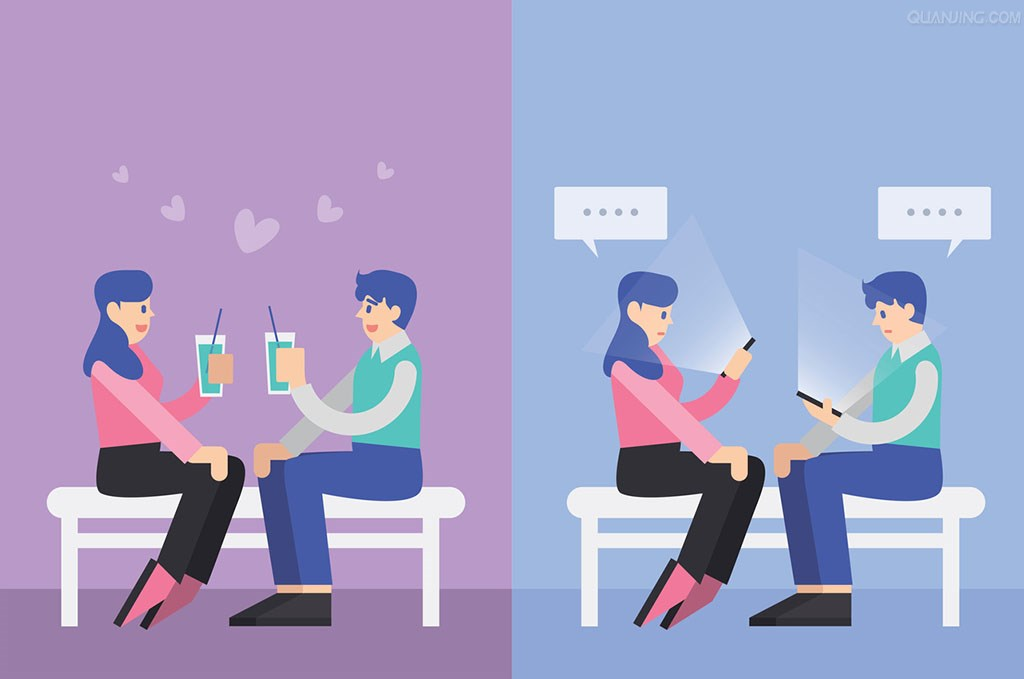
\includegraphics[width=0.495\paperwidth]{ti279a0209}
		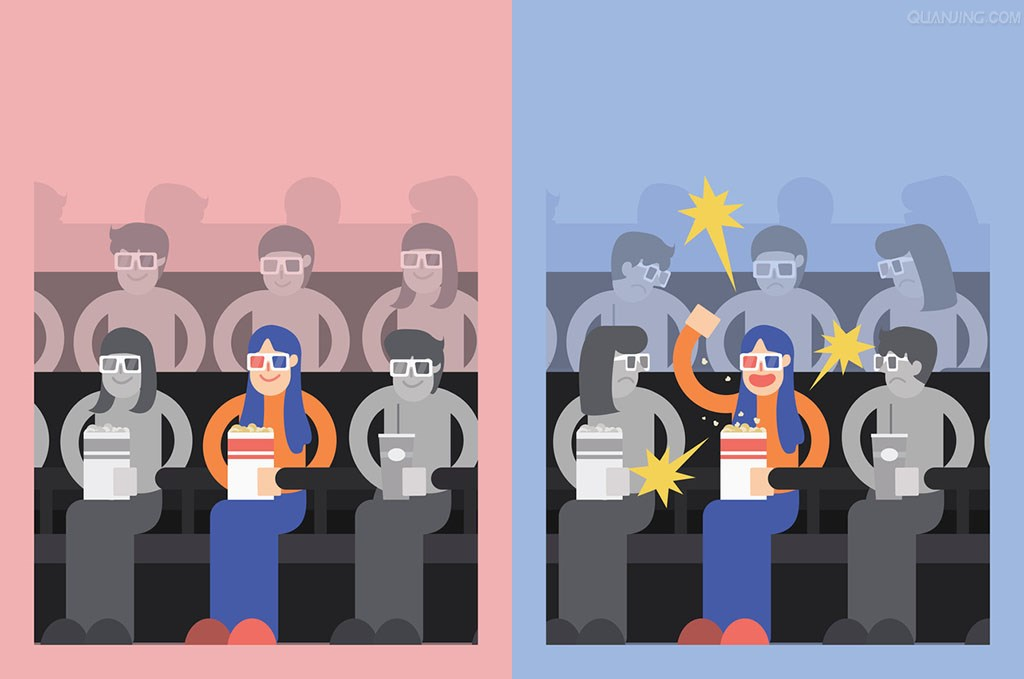
\includegraphics[width=0.495\paperwidth]{ti279a0205}
	\end{center}
\end{textblock}

\begin{textblock}{1}(0,.53)
    \begin{center}
        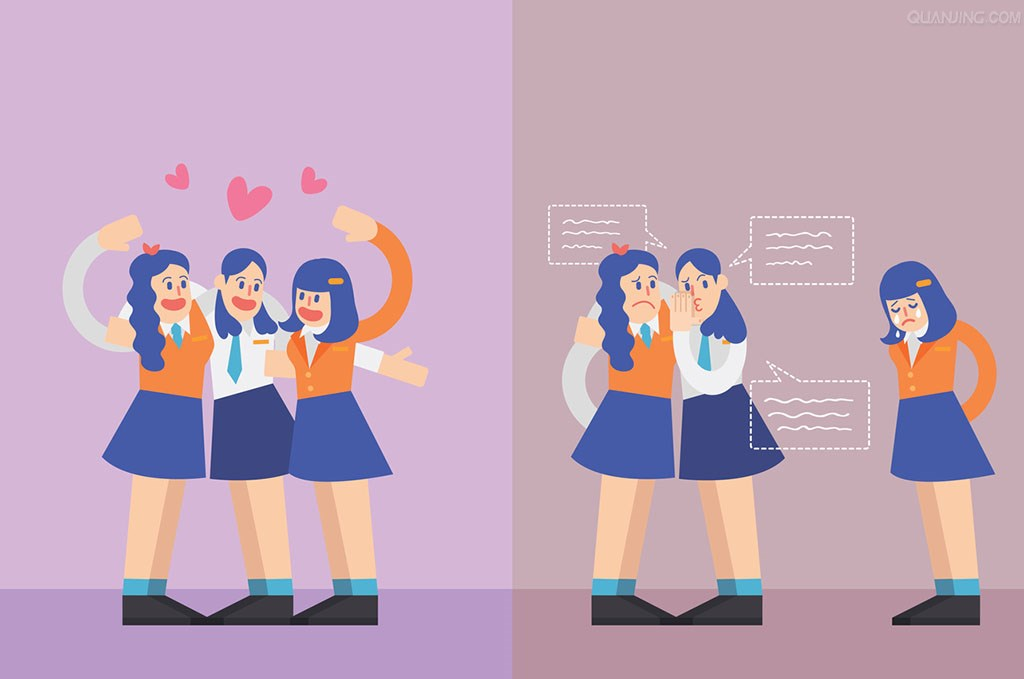
\includegraphics[width=0.495\paperwidth]{ti279a0217}
        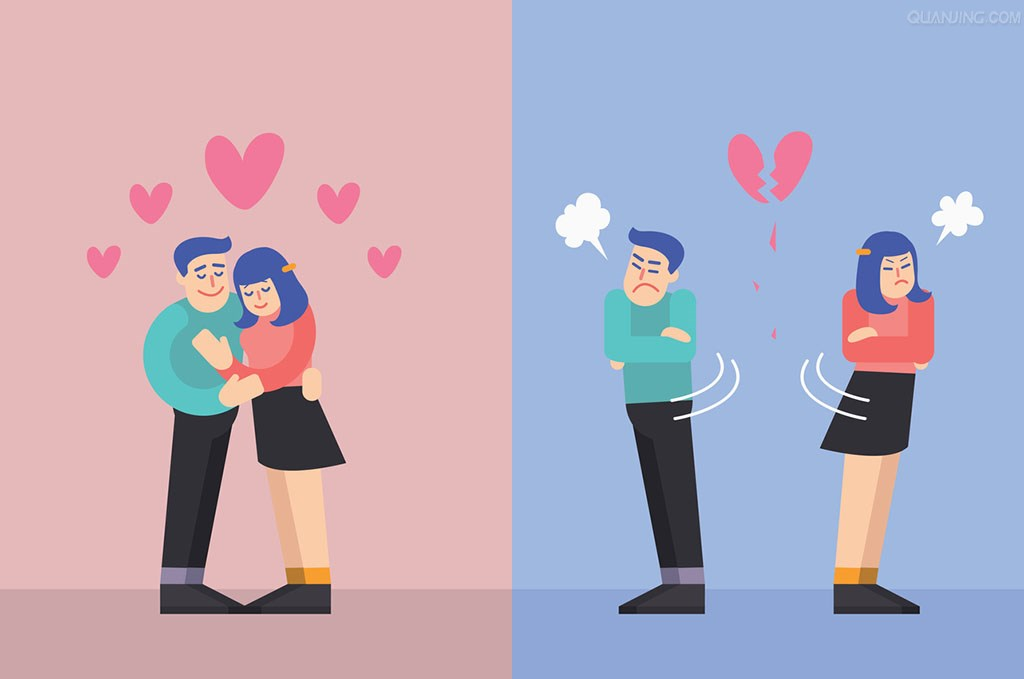
\includegraphics[width=0.495\paperwidth]{ti279a0206}
    \end{center}
\end{textblock}

\begin{textblock}{1}(0,.76)
	\begin{center}
		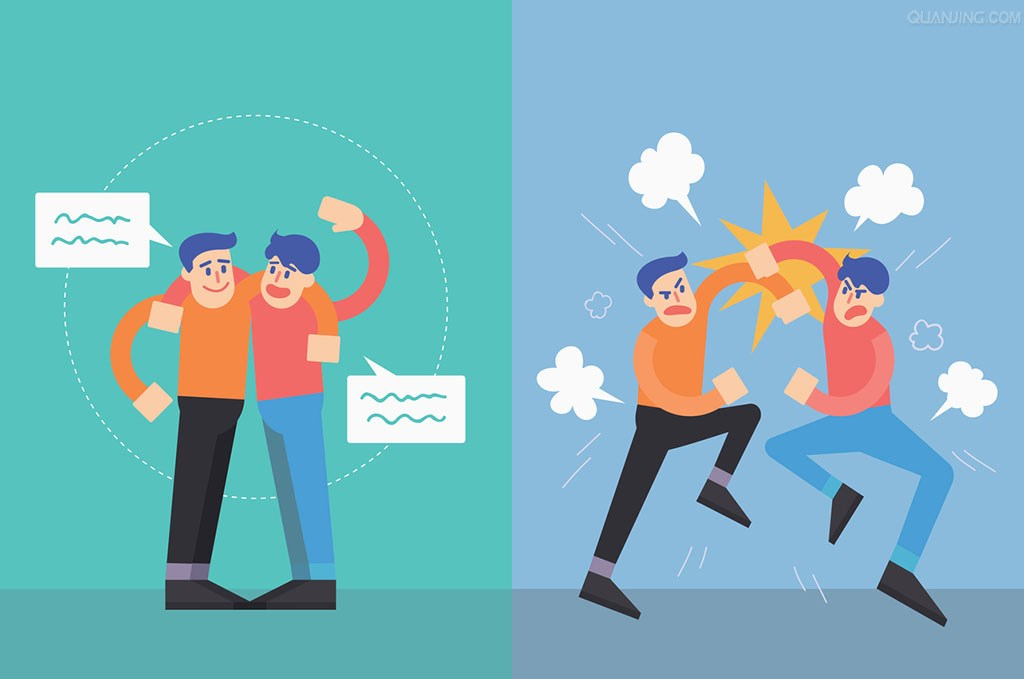
\includegraphics[width=0.495\paperwidth]{ti279a0201}
		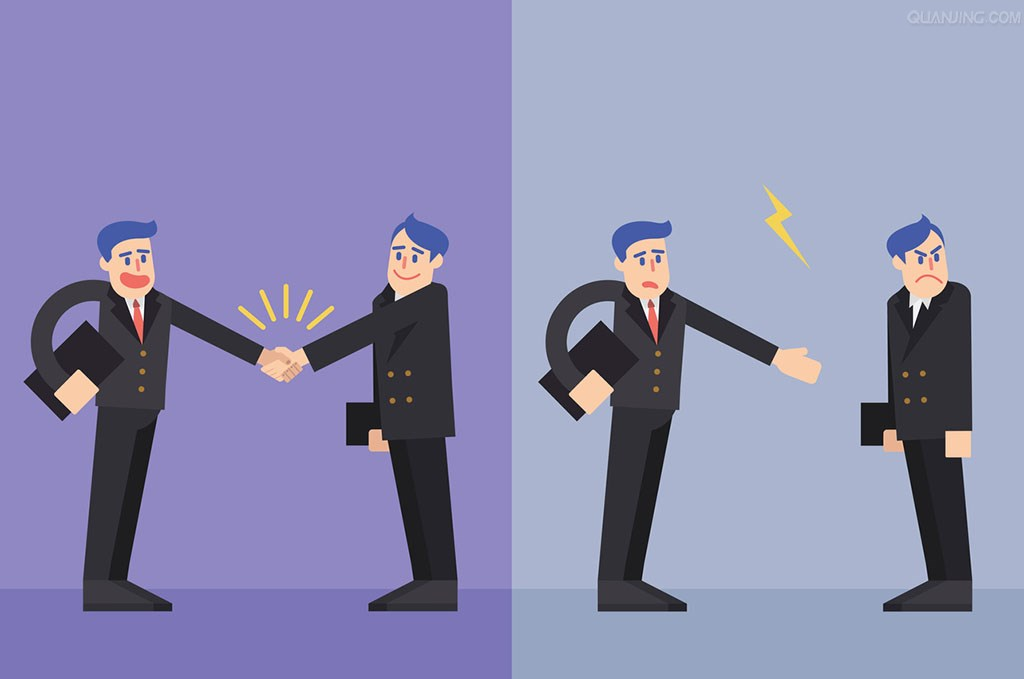
\includegraphics[width=0.495\paperwidth]{ti279a0207}
	\end{center}
\end{textblock}

%\begin{textblock}{1}(.3,0.95)
%	\noindent{\fontsize{20.74}{2}\selectfont
%		\bfseries\textcolor{blue}{2017年3月18日}}
%\end{textblock}
%\begin{textblock}{.4}(.05,.65)
%    \begin{center}
%        \includegraphics[width=.4\paperwidth]{arccos}
%    \end{center}
%\end{textblock}
\null\newpage\pagestyle{nexus}

\tableofcontents

\chapter{申请篇}

\section{为什么你没通过我的好友申请}
\begin{tcolorbox}[colback=orange!5,colframe=orange!75!black]
\begin{enumerate}
	\item \textcolor{red}{人们倾向于记住最先发生的事情和最后发生的事情}。中间的事情记不清楚。所以,如果你要做自我介绍的话,最好做第一个或者最后一个。面试的时候,也是一样的。
	\item \textcolor{red}{如果你在酒吧或者前台工作,在你身后放一面镜子}。这样的话,当顾客发脾气的时候,就能从镜子里看到自己的丑恶嘴脸。一面镜子可以显著降低他们无理取闹的概率。
	\item \textcolor{red}{报价之后,不再说话}。如果你是做销售工作的,这项技巧很有用。在其他领域,这项技巧也很有用。我之前干过一份工作,是在一家体育馆卖会员卡。有个老家伙就是这么指导我的,他说,一旦你和顾客寒暄完毕,报出了你的价格。从此时开始,先开口的那个就输了。看起来好像毫无根据,但确实是这个样子的。通常会有很长时间的尴尬沉默,但是,最终,顾客会买的。
\item \textcolor{red}{如果你问了别人一个问题,然后他们回答了一半,你等着,他们会说完的}。只要等着,保持眼神接触,最终,他们会开口讲完的。
\item \textcolor{red}{公开讲话或者蹦极之前这种会紧张的时刻,嚼口香糖就好了}。据说是因为人类在危险的时候会自动停止咀嚼(吃东西),所以吃东西的时候就是安全的,大脑就是这么告诉你的。反正这招对我很管用。
\item \textcolor{red}{人们最终记住的不是你说过的话},而是你让他们产生的感觉。几乎所有的人都喜欢谈论自己的事情,所以,多问问题。
\item \textcolor{red}{当你学习新东西的时候,尝试着教给朋友们,或者让他们问你相关的问题}。如果你能教给人一杯水,你自己一定会有一桶水。
\item \textcolor{red}{如果你看到某人时,很开心,溢于言表的开心,那么他们以后看到你也会手舞足蹈的}。第一次也许不是这样,但第二次一定是。
\item \textcolor{red}{身体对压力的反应——呼吸加速,心跳加快——和鼓起勇气时的反应是一样的}。所以是好是歹,全在你一念之间。反正你的身体已经都准备好了,你看着办吧。
\item \textcolor{red}{注意别人的脚。当你加入别人的谈话时,发现别人只是把上半身转过来了,脚还是维持原来的方向,那就说明他们不欢迎你的加入}。类似的,你和你的同事谈话时,你觉得他在专心和你谈话,他的身体也面向你,但他的脚却不是朝向你的,他可能早就已经受不了这场谈话了。
\end{enumerate}
\end{tcolorbox}
\begin{tcolorbox}[colback=orange!5,colframe=orange!75!black]
	\begin{enumerate}
\item \textcolor{red}{装出牛逼的样子,直到你做到了};信心比知道更重要。别被任何人吓住,生活不易,全靠演技,那些吓你的人也在演戏。
\item \textcolor{red}{你假装成什么样子,你最终就会成为什么样子}。装逼得逼,求仁成仁,念念不忘,必有回响。
\item \textcolor{red}{虽然不是要你去吓人,但如果你一定要厚颜无耻的盯着某人,视线聚集在他的两只眼睛中间,等着他们害羞}。如果他们移开视线,他们就不会再看着你。这个时候,你就可以肆无忌惮的盯着他们的眼睛了。至少有45秒的时间哦。
\item \textcolor{red}{建立人际网络。成为朋友们的信息源},当然,他们也会是你的信息源。和前同事一起喝杯酒吧,也是好的。
\item \textcolor{red}{如果你前面的车子慢的像是老爷爷在开,你恨不得杀了他。假装他真的是你的亲爷爷。 然后你的怒气就全消了}。
\item \textcolor{red}{站得直}。 不许没精打采,不许手插兜,头要高高抬起。不要觉得这是陈词滥调。你自己会因此觉得很好,而且周围的人也会感受到你的自信。
\item \textcolor{red}{不要说“我觉得”、“我认为”},除非真的有必要。这些词语会让你和自信无缘,对你可没什么好处。
\item \textcolor{red}{焦虑的时候,收拾一下家里或者工作桌}。你会比之前更开心、更有感觉。
\item \textcolor{red}{第一次饭,第一支酒,你请}。你都不知道你自己会因此而自我感觉良好多久。
\item \textcolor{red}{为人父母者请注意:给孩子们选择的权利,让他们认为自己掌控自己的生活}。比如我想让孩子自己穿鞋的时候,我会问他“你是想穿那双星星的,还是鲨鱼的?”。值得注意的是,这招对成年人也管用。
\item \textcolor{red}{态度决定行动,可是行动也决定态度}。就像我以前的一个老师说的那样:你可以因为高兴而跳起舞来,也可以故意跳起舞来让自己高兴。
\item \textcolor{red}{一群人在大笑的时候,人们会立刻看向这群人里最亲近的人}。
\item \textcolor{red}{如果你想和某人建立密切的关系,或者获得某人的信任,学习他的身体的姿势}。如果他翘起二郎腿,你也翘起来。如果他斜靠在椅背上,你也斜靠在椅背上,如果他身体前倾,你也身体前倾。模仿身体姿势,是一种下意识的信任对方和自在的表现。如果你在胸前交叉双臂时发现某人随即也这么做了,恭喜你,你又迷住了一个人。

\item \textcolor{red}{本杰明·富兰克林效应。在学生时代},找女生借铅笔、借笔记、求她帮你补习功课,比起借给她东西、帮她补习功课,女生更容易爱上找她借铅笔的那个穷/笨小子。调情的时候这也很有用,比如(开玩笑似的)让女孩请你喝支酒。这可是一石三鸟的事情:你得到了好处;她会下意识的更喜欢你;将来她接受你的“帮助”也会更加没有负担。

\end{enumerate}
\end{tcolorbox}

\chapter{工作}
\begin{tcolorbox}[colback=orange!5,colframe=orange!75!black]
	\begin{enumerate}
\item  当你准备演讲的时候,永远在桌子上放一瓶水。当你突然想不起来该说啥的时候,喝口水。听众不会感到任何异常的。
\item  在电器商店里找不到人为你讲解么?那就站在最贵的电视机前,盯着价格标签看。马上会有人屁颠屁颠地出现的。
\item  怀疑有人在跟踪你的车?那就来四个右转弯吧!这样,你的行驶路线可以形成一个圈。如果那个家伙还在,那他肯定在跟踪你。
\item 如果你害怕有人会偷走你的蓝色钢笔,就给它安上一个红色的笔帽,因为没有人会偷一支红色的钢笔的。
\item  如果你在公众场合被发现做了一件令人尴尬的事情,没关系,就说你在玩“真心话大冒险”。
\item 15分钟的大笑,等同于30分钟的仰卧起坐。
\item  在商店里,最便宜的东西不是在最上面的货架,就是在最下面的货架,而不会在眼睛的水平线上。
\item 当你保存你的ppt时,用后缀.pps或.ppsx,那样的话,打开时会直接进入幻灯片播放模式。不仅节省时间,还看起来十分专业。
啊,这个技巧10秒钟就可以学会了哦~
*(亲测有效)*
\end{enumerate}
\end{tcolorbox}

\begin{proposition}[生活情调]
以下行为你*只需要花3秒钟*,但你一定会爱上它的!

步骤1:把你的手机从口袋里掏出;

步骤2:录下你眼前的一个很短的瞬间;

步骤3:每天重复;

步骤4:把你每天录下的东西剪辑成1秒,并把它们接在一起。

这样的话,每年的年终,你可以看到一个大约6分钟的录像,它是你当年生活的浓缩。
时间机器并不存在,但这个方法是最好的替代品。每一秒的播放,都会让你的记忆闪回到你年轻时的那一瞬间,它记录了你在世界留下的印痕。

你会记得你在沙滩上的性感瞬间,会记得那个除了吃方便面以外无事可做的百无聊赖的日子,或者在雨后那一轮美丽的彩虹。

所有的东西,都最生动而真实地展现出来了。

\end{proposition}
\chapter{学习}
\begin{proposition}[生活情调]
	这更像是一条忠告:*晚上,请把你的汽车钥匙放在床边。*
	
	如果你听到房外有喧闹声,或者有人试图有人进入你的房间,马上按下你汽车的报警按钮。警报会响起,直到你关闭按钮或者汽车没电。
	
	当汽车警报响起时,如果有人尝试闯入你的房间,他绝对不敢逗留,因为过不了多久,大部分邻居都会出来看到底发生了什么。有时候,这个小技巧会拯救一条生命,或者一个潜在的性犯罪。
\end{proposition}

\begin{tcolorbox}[colback=orange!5,colframe=orange!75!black]
\begin{enumerate}
\item 需要记住在离家之前必须带的东西?把它放在鞋子里,你肯定不会忘记穿鞋的。
\item 无法确定自己是否饿了?问一下自己是否需要一个苹果。如果答案是“不”,那么你可能不是饿了,而是无聊了。
\item 避免用very这个单词。这大概是英语中最被滥用的单词,因为very用于强调动词、形容词和副词都是很方便的。但是,用一个单词来清晰地表达你的想法,会让你显得更聪明哦!
\item 在你孩子还小的时候,给他们创建一个email的账号,坚持给那个账号发送图片和任何有价值的东西。等他们长大后 ,告诉他们email账号的密码,他们一定会很喜欢的。
\item 如果你感觉到有类似于灰尘的东西在你眼睛里,那就这样做:
*向下看,睁大眼睛,不断眨眼。*
另外,如果那玩意儿顽固不化,那就移动你的眼球:朝着你感觉痛的位置的反方向移动。所以如果是顶部感到痛,那就按照上面的步骤做,不过要把你的眼球底部移动。		
\end{enumerate}
\end{tcolorbox}
\chapter{生活}
\begin{proposition}[追狗狗]
如果你和小狗狗散步时,她跑开了,千万别吼完她后追她,她会觉得这是世界上最好玩的游戏……嗯,追狗愉快!
你应该欢快地叫道:“嘿,欢欢,你抓不到我!”然后像个疯狂的傻逼一样往另一个方向跑去,你的小狗狗会觉得你很享受这种感觉 ,然后在你的背后追你。
然后,一旦她重新来到了你的背后,不要责骂她的淘气。如果你这么做了,她会以为你觉得她不该回来,而不是不该擅自跑远,这样的话,下次她跑远的时候就更不愿意回来了。你应该对她的归来表示友好
\end{proposition}
\chapter{社交}
\begin{proposition}[缓解压力]
*感到压力太大?这种感觉让你无法学习和工作?或者感到自己的头快炸了?或者你感到自己能力不够,快要放弃了?*

试试这些:

切断你的网络连接。

* 穿上你的跑鞋,戴上耳机放着你最喜欢、最有节奏感的音乐,立刻、马上去跑步。跑得越快越好,越远越好。

* 如果你不能出去跑步,做10个俯卧撑、10个仰卧起坐、10个深蹲,然后再一个地方踱步一分钟,再做一组。

* 洗个痛快澡。

* 为自己做一杯热咖啡。

* 听一些软软的音乐。

* 啊,压力融化了哟!

这并不是从网上复制下来的。这是一个被尝试和测试过的方法,能很快冷静下来。
\end{proposition}

\begin{proposition}[西餐礼仪]
	当我是个孩子的时候,餐桌礼仪让我感到很迷惑。我不知道在吃饭的时候用哪个手该做什么。后来,我发现了一个小技巧。
	左(Left,4个字母)手边放4个字母的东西——叉子(fork);
	右(Right,5个字母)手边放5个字母的东西——调羹(spoon),刀(knife),玻璃杯(glass)
	
\end{proposition}
\chapter{购物}
\begin{proposition}[购物须知]
	如果你要去购物商场或者超市,千万不要*空腹*去。而是,先吃点东西,然后再去。理由是,当你满足了你的胃,你的精神也会得到满足,这将防止你去买一些你并不需要的东西。你将会买那些需要的商品,因为你已经感觉良好了。我曾经试过很多次,每当我和我的女朋友要去商场前,我更倾向于先去餐馆。(哭)
\end{proposition}
\chapter{搜索}

\chapter{冷知识}
\begin{proposition}[苏格拉底的“三过滤”]
	在古希腊,一天某人遇到了伟大的哲学家苏格拉底,他问道“你知道我从朋友那里听到了什么吗?"
	
	"先等一会儿”,苏格拉底答道,“在你告诉我任何事情之前,我需要你通过一个小小的测试 。它叫做‘三过滤’测试。”
	
	“三过滤?”
	
	“是的,” 苏格拉底答道,“在你告诉我关于你朋友的事情之前,最好等一下,然后过滤一下你说的东西。所以我叫它三过滤测试。
	
	“第一个过滤器是*真实(Truth)*。你是否确定你要告诉我的东西是真的吗?”
	
	“并不。”那人说,“事实上我只是从朋友那里听说并且……”
	
	“好的,”苏格拉底说,“所以你并不知道那是否正确。接下来是第二个过滤器,叫做*善意(Goodness)*,你要告诉我的关于你朋友的事情是好事吗?”
	
	“不,与之相反……”
	
	“所以,”苏格拉底继续道,“你将告诉我一些关于他的坏消息,但你不能保证它是正确的。
	
	“你将继续你的测试,因为还有一个过滤器呢,它叫*有用(Usefulness)*。你要告诉我的关于你朋友的事情对我有用吗?”
	
	“不,我想不是。”
	
	“好了,”苏格拉底继续说道,“*如果你要告诉我的东西既不一定真实,也不是好消息,甚至都没用,那你TMD究竟为何要告诉我?*”
	
\end{proposition}

\begin{proposition}[女性合乘修正]
在IRCTC(印度铁路)坐车时,我总是预定两个座位,并在几天以后取消其中一个。一个座位用我的名字,另一个座位用一个(假的)女孩名字,这样的话,另一个座位最终也会是女乘客。这就是IRCTC算法工作的方式,我们称其为 女性合乘修正(female co-passenger hack)。
\end{proposition}

	
\end{document}

